%%%%%%%%%%%%%%%%%%%%%%%%%%%%%%%%%%%%%%%%%%%%%%%%%%%%%%%%%%%%%%%%%%
% Sample template for MIT Junior Lab Student Written Summaries
% Available from http://web.mit.edu/8.13/www/Samplepaper/sample-paper.tex
%
% Last Updated August 30, 2011
%
% Adapted from the American Physical Societies REVTeK-4.1 Pages
% at http://publish.aps.org
%
% ADVICE TO STUDENTS: Each time you write a paper, start with this
% template and save under a new filename. If convenient, don't
%    erase unneeded lines, just comment them out.  Often, they
%    will be useful containers for information.
%
% Using pdflatex, images must be either PNG, GIF, JPEG or PDF.
%     Turn eps to pdf using epstopdf.
%%%%%%%%%%%%%%%%%%%%%%%%%%%%%%%%%%%%%%%%%%%%%%%%%%%%%%%%%%%%%%%%%%


%%%%%%%%%%%%%%%%%%%%%%%%%%%%%%%%%%%%%%%%%%%%%%%%%%%%%%%%%%%%%%%%%%
% PREAMBLE
% The preamble of a LaTeX document is the set of commands that precede
% the \begin{document} line.  It contains a \documentclass line
% to load the REVTeK-4.1 macro definitions and various \usepackage
% lines to load other macro packages.
%
% ADVICE TO STUDENTS: This preamble contains a suggested set of
% class options to generate a ``Junior Lab'' look and feel that
% facilitate quick review and feedback from one's peers, TA's
% and section instructors. Don't make substantial changes without
%     first consulting your section instructor.
%%%%%%%%%%%%%%%%%%%%%%%%%%%%%%%%%%%%%%%%%%%%%%%%%%%%%%%%%%%%%%%%%%

\documentclass[aps,twocolumn,secnumarabic,balancelastpage,amsmath,amssymb,nofootinbib]{revtex4}
%\documentclass[aps,twocolumn,secnumarabic,balancelastpage,amsmath,amssymb,nofootinbib]{revtex4-1}
\pdfpagewidth 8.5in
\pdfpageheight 11in

\usepackage{lgrind} % convert program listings to a form includable in a LaTeX document
\usepackage{chapterbib} % allows a bibliography for each chapter(each labguide has it's own)
\usepackage{color} % produces boxes or entire pages with coloredbackgrounds
\usepackage{graphics}      % standard graphics specifications
\usepackage[pdftex]{graphicx} % alternative graphics specifications
\usepackage{longtable}     % helps with long table options
\usepackage{epsf} % old package handles encapsulated post scriptissues
\usepackage{bm}            % special 'bold-math' package
%\usepackage{asymptote} % For typesetting of mathematical illustrations
\usepackage{thumbpdf}
\usepackage[colorlinks=true]{hyperref} % this package should be added after all others
% use as follows: \url{http://web.mit.edu/8.13}
\usepackage{multirow}
\usepackage{subfigure}

% Define a useful new command for writing units
\newcommand{\cd}{$\cdot$}

%
% And now, begin the document...
%

\begin{document}
\title{Spin-Lattice Relaxation}
\author{Jay M.\ Lawhorn}
\email{klawhorn@mit.edu}
\date{\today}
\affiliation{MIT Department of Physics}

\begin{abstract}
A study of spin-lattice relaxation effects in nuclear magnetic resonance measurements is presented. The gyromagnetic ratio of $^1$H is measured at $26.8\pm0.5$ rad kHz/G. Several basic radio frequency (RF) sequences composed of $\pi/2$ and $\pi$ pulses are used in samples consisting of various combinations of glycerine and water to measure the spin-lattice time constant, $T_1$. The $T_1$ of glycerine is measured to be $29.6\pm3.7$ms, and for water $2.12\pm0.27$s. 
\end{abstract}

\maketitle

The nuclear magnetic resonance (NMR) method is widely used in a variety contexts from medical imaging to molecular physics and chemistry to quantum computing. This paper describes a series of experiments using pulsed NMR techniques. To study each sample, it is placed inside a solenoid in a large static magnetic field. The inductor coil is then used to apply a known radio frequency (RF) signal to the sample under study for a set amount of time. The RF signal creates a small oscillating magnetic field, which can be treated as a perturbation to the system in time-dependent perturbation theory. 

Spins in a static magnetic field will precess about an axis in the direction of the magnetic field (equilibrium axis). This precession frequency is fixed for each nucleus and is known as the Larmor frequency, $\omega_{\mathrm{L}}$. It is given by  
\begin{equation}
\omega_{\mathrm{L}} = \gamma B_{0}
\label{eq:gamma}
\end{equation}
where $\gamma$ is the gyromagnetic ratio of the nucleus and $B_{0}$ is the magnitude of the magnetic field.

When the applied magnetic field oscillates at or near the Larmor frequency in a direction perpendicular to the equilibrium axis, the spins will rotate about the axis of the applied magnetic field, with the pulse length determining how far the spin rotates. A pulse long enough to rotate a spin along the equilibrium axis to point exactly along the inverse axis is called a $\pi$ pulse. Similarly, a pulse applied for half the time of a $\pi$ pulse is called a $\pi/2$ pulse and will rotate a spin along the equilibrium axis into the plane perpendicular to the static magnetic field. 

In the same way that the applied RF pulse produces an oscillating magnetic field in the solenoid volume, spin rotations in the plane induce an electric current in the solenoid. These induced currents create the observed signals, which can be classified into two main forms, both of which are shown in Figure \ref{fig:fidecho}.

The first is a free induction decay (FID), which is an oscillatory signal damped by an exponential decay. Its envelope is determined by the inhomogeneities in the magnetic field that cause spins in different parts of the sample to precess at slightly different frequencies, decreasing the overall magnetization of the sample.

The second is a spin echo, which occurs when spins in the plane are rotated by a $\pi$ pulse. The spins return to the plane, but are inverted. Spins that were precessing faster than average before will be behind the average after, creating a point where the effect of inhomogeneities in the magnetic field are exactly canceled. This point corresponds to the maximum of the observed spin echo.

\begin{figure}[htb]
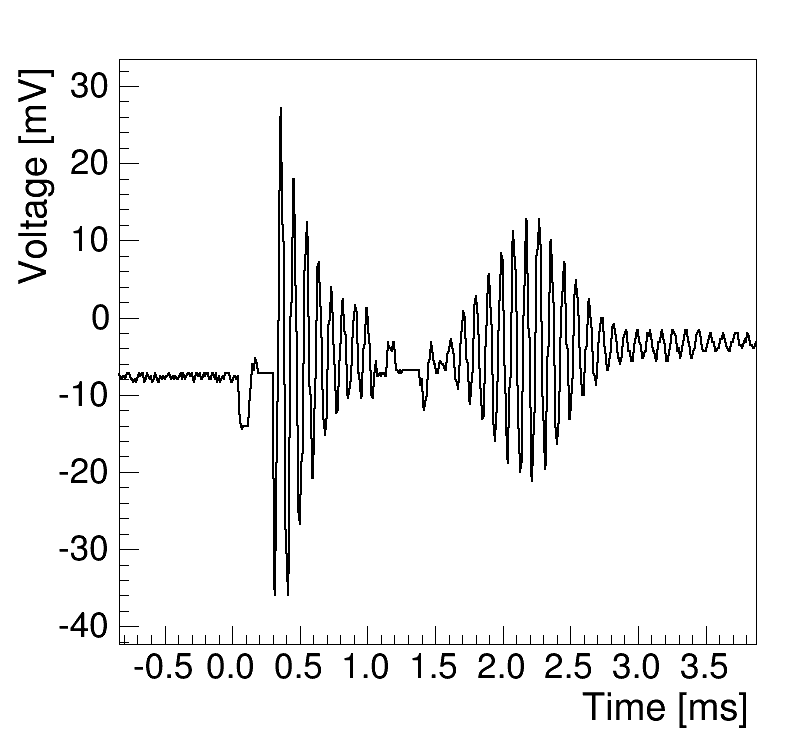
\includegraphics[width=6cm]{water_n2/fidecho.png}
\caption{This waveform shows a free induction decay (FID) followed by a spin echo. Note that the spin echo amplitude is smaller than the FID, due to thermal relaxation effects.}
\label{fig:fidecho}
\end{figure}

Spin-lattice relaxation, or longitudinal relaxation, is one of three major relaxation effects in NMR. It describes the sample's return to thermal equilibrium after spins are rotated away from the equilibrium axis by a RF pulse. In room temperature liquid samples like glycerine and water, dipole-dipole interactions dominates the spin-lattice relaxation time\cite{ray}. Dipoles in the surrounding media produce small oscillatory magnetic fields and if these magnetic fields happen to be oscillating at frequencies near the Larmor frequency they will interact with the dipoles under study.

The efficiency of dipole-dipole interactions increases with the viscosity of the substance because the Larmor frequency is generally very slow compared to molecular tumbling in liquids. Since only oscillations at frequencies near the Larmor frequency contribute to relaxation, substances with slower average molecular tumbling will have a larger component near resonance, and the average molecular tumbling speed is directly related to the viscosity of the substance. Thus substances with low viscosity, such as water, are expected to have longer spin-lattice relaxation times than higher viscosity substances like glycerine.

The speed of thermal relaxation through the dipole-dipole interaction is expected to vary based on the surrounding magnetic environment. Water generally contains significant amounts of dissolved oxygen, which is paramagnetic. Water containing dissolved nitrogen, which is diamagnetic, is expected to relax slower than water with dissolved oxygen because there is a much weaker coupling to the environment.

The apparatus consists of a permanent magnet that produces a static magnetic field and a probe circuit that delivers a radio frequency (RF) pulse and detects the resulting signal. A schematic of the apparatus is shown in Fig \ref{fig:app}.

\begin{figure}[htb]
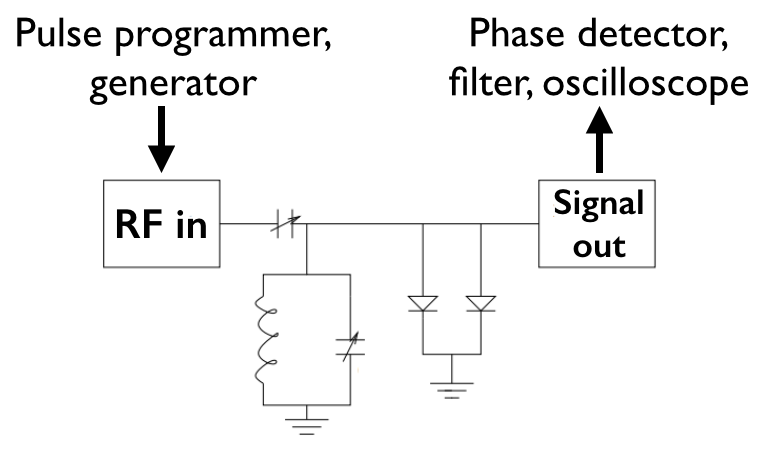
\includegraphics[width=6cm]{apparatus.png}
\caption{The sample is enclosed in a ten-turn copper coil that both delivers the applied RF pulse and transmits the resulting signal. A pair of crossed diodes protect the pre-amplifier from the large RF pulses but allows the small signal currents to pass. The capacitors are appropriately tuned for impedance matching with the rest of the signal chain.}
\label{fig:app}
\end{figure}

The RF pulses are generated by a frequency synthesizer and fed through a power splitter which sends half of the signal to a double-balanced mixer and the other half to a phase detector for the output. The double-balanced mixer serves as a gate for the RF signal and is controlled by a digital pulse programmer which sets the pulse widths and timings. The RF signal is then amplified and sent to the probe circuit. 

The induced current from the magnetization of the sample is fed through a pre-amplifier and then mixed with the synthesized frequency. The difference signal from the mixer is then read out on an oscilloscope.

The static magnetic field was measured at $1760\pm30$ G using a Hall magnetometer. The magnetometer was calibrated with a zero gauss chamber, and a $202.5 \pm 1\%$ test probe to $1.9\%$ accuracy. The raw magnetometer reading inside the test coil to available precision was $1.762\pm0.005$ G. The uncertainty in magnetic field was taken to be the uncertainties from the precision of the magnetometer and the accuracy of calibration added in quadrature.

The Larmor frequency of the material was determined by visual inspection of the signal after an RF pulse as the input frequency was varied. The Larmor frequency was identified as the frequency that minimized the observed beat pattern. 

The Larmor frequency of hydrogen in glycerine was measured as $7.5210\pm0.0001$ MHz, with the uncertainty assessed based on our ability to distinguish differences in beat patterns on the oscilloscope. The Larmor frequency of fluorine in a fluropolymer was measured as $7.076\pm0.002$ MHz, with uncertainty again limited by visual observation of the beat patterns.

The gyromagnetic ratio of each sample was calculated using Eq \ref{eq:gamma} with linear error propagation of the uncertainties
on the Larmor frequency and magnetic field strength. For hydrogen, $\omega_{\mathrm{L}}=26.8\pm0.5$ rad kHz/G, and for fluorine $\omega_{\mathrm{L}}=25.2\pm0.5$ rad kHz/G. Both measurements are in agreement with the literature values of 26.8 and 25.2 rad kHz/G respectively\cite{crc}.

It is crucial to set the RF frequency for the applied pulses close to the Larmor frequency but not exactly at it, because all measurements of FIDs and spin echos depend on the beat patterns. These beat patterns vanish at the Larmor frequency, making observations difficult or impossible. For the measurements described below in glycerine we chose to set the frequency to 5.523MHz, only 2kHz away from the measured Larmor frequency of hydrogen. However, upon analysis this frequency did not create a sufficiently fast beat pattern, so for the subsequent measurements in glycerine solutions and water we set the frequency to 7.531 MHz to decrease our systematic uncertainties related to amplitude extraction on waveforms.

The pulse width for a $\pi$ pulse was determined to be the pulse width in microseconds that minimized the resulting free induction decay. The $\pi/2$ pulse width was then taken to be half the $\pi$ pulse width. These pulse widths were determined each day and $\pi$ pulses typically fell within 40-60$\mu$s. Each $\pi$ pulse width determination had an uncertainty of 5$\mu$s. The uncertainty introduced in the following measurements by the pulse widths was neglected because the response magnetization in the plane is proportional to $\sin(\mathrm{PW})$ and a 10\% uncertainty on the $\pi/2$ pulse width corresponds 2\% uncertainty on the magnitude of FID. While this is on the same order as our reported uncertainties, it is the same for all measurements made in a set, and while it should be taken into account for precision measurements and long chains of pulses, it is neglected here.

All fits were made using ROOT's built-in fit functions and $\chi^2$ minimization. In all measurements described below, there is some expected term that goes as $\mathrm{exp}(b\tau)$. $T_{1}$ was taken to be $1/b$, and the reported uncertainty on the fit parameter $b$ was linearly propagated to calculate an uncertainty on $T_{1}$ using the formula $dT_{1}=db/b^{2}$.

Three different pulse sequences for the determination of the spin-lattice relaxation time were used in glycerine: $\pi/2$-$\tau$-$\pi/2$, $\pi$-$\tau$-$\pi/2$, and $\pi/2$-$\tau$-$\pi/2$-$\pi$. 

For the $\pi/2$-$\tau$-$\pi/2$ sequence, the spins at the equilibrium axis are rotated into the plane by the first $\pi$/2 pulse, and the system is allowed to relax for a variable time $\tau$. The second $\pi/2$ pulse rotates all spins that have returned to the equilibrium axis back into the plane and all spins still in the plane to the inverted axis, resulting in a FID with magnitude proportional to the fraction of spins that relaxed back to equilibrium in a time $\tau$. The magnitude of the FID is expected to go as $A(1-\mathrm{exp}(-\tau/T_{1}))$ where $A$ is the maximal FID amplitude, and $T_{1}$ is the spin-lattice relaxation time.

For each $\tau$, three measurements were taken with 25$\mu$s $\pi/2$ pulses, and a repeat time of 200ms. The FID amplitude was measured by hand, aligning the oscilloscope cursors with the highest and lowest peak of the FID and recording the reported difference between the two cursors. The uncertainty on each amplitude was taken to be 1.1mV due to the resolution of the cursor placement. The three measurements were averaged, and the overall uncertainty for each tau was taken as the standard deviation of the measurements added in quadrature with the systematic uncertainty from the cursor placement and divided by the square root of the number of measurements. 

A fit of the form $a-\mathrm{exp}(b\tau-c)$ was made to the data. The measured $T_1$ for glycerine was $30.9\pm4.5$. 

For the $\pi$-$\tau$-$\pi/2$ sequence, the spins at the equilibrium axis are first inverted by the $\pi$ pulse, and the system is allowed to relax for a variable time $\tau$. The $\pi/2$ pulse rotates all spins that have returned to the equilibrium axis and any spins remaining at the inverted axis back into the plane. This means that the FID amplitude will go through a minimum where the majority of the spins are in the plane when the second pulse was applied. Because our apparatus cannot distinguish if pulses rotated into the plane come from the equilibrium axis or the inverted axis, the observed FID amplitude is expected to go as $A|1-2\mathrm{exp}(-\tau/T_{1})|$ where $A$ is the maximal FID amplitude, and $T_{1}$ is the spin-lattice relaxation time.

For each $\tau$, three measurements were taken with 25$\mu$s $\pi/2$ pulses, and a repeat time of 200ms. The FID amplitude was measured by hand and processed using the same techniques described for the $\pi/2$-$\tau$-$\pi/2$ sequence. 

The first recorded point at $\tau=4$ was excluded in order to simplify the fit expression by removing the absolute value and need to fit to an additional parameter describing the zero point in the data. The fit used was of the form $a-\mathrm{exp}(b\tau-c)$. Excluding the first point was effectively choosing the range in which the minimum of the full curve falls. To estimate the systematic uncertainty introduced by setting it between the first and second points, a second fit of the same form was performed excluding the first two data points. The difference between the two values was taken as a systematic uncertainty on $T_{1}$. The uncertainty on the fitted parameter was linearly propagated to calculate the uncertainty on $T_{1}$ from each fit. The single-exclusion fit is shown in Figure \ref{fig:18090} and was chosen to minimize the calculated fit uncertainty on the nominal value of $T_{1}$.

\begin{figure}[htb]
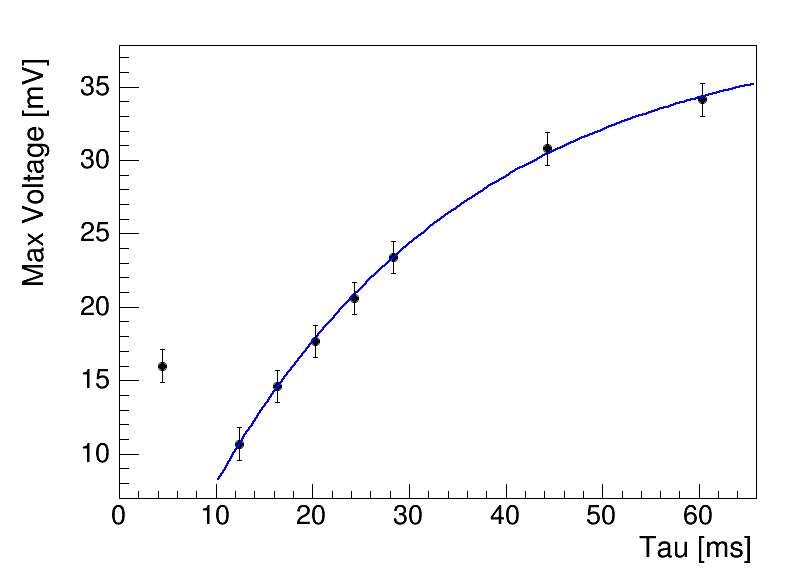
\includegraphics[width=6cm]{images/t1_180t90.png}
\caption{FID amplitude as a function of delay time $\tau$ between two pulses in the $\pi$-$\tau$-$\pi/2$ sequence. The nominal fit excluding only the first data point is shown.}
\label{fig:18090}
\end{figure}

The measured $T_1$ for glycerine using the $\pi$-$\tau$-$\pi/2$ sequence was $27.1 \pm 6.2\mathrm{(fit}) \pm 0.92 \mathrm{(exc)}$.

The $\pi/2$-$\tau$-$\pi/2$-$\pi$ sequence is the same as the $\pi$-$\tau$-$\pi/2$ sequence with an extra $\pi$ pulse is applied shortly after the second pulse. This third pulse inverts all spins, leaving spins in the plane in the plane but rotated by $\pi$, creating a spin echo following the third pulse by exactly the delay between the second and third pulses. The observed spin echo amplitude is expected to go as $A|1-2\mathrm{exp}(-\tau/T_{1})|$ where $A$ is the maximal spin amplitude, and $T_{1}$ is the spin-lattice relaxation time.

For each $\tau$, three measurements were taken with 24$\mu$s $\pi/2$ pulses, and a repeat time of 200ms, with a pulse frequency of 7.253 MHz. The oscilloscope output was saved as a text file and processed. For each waveform, the measurement uncertainty was taken to be the standard deviation of the recorded values for the first 1000 data points, comprising 0.8ms of noise recorded well before the first RF pulse was applied. The calculated uncertainties fell between 0.2-0.4mV. The three measurements were averaged, and the overall uncertainty for each $\tau$ was taken as the standard deviation of the measurements added in quadrature with the calculated uncertainties based on waveform noise divided by the square root of the number of measurements.

The spin echo amplitude was calculated as the difference between the maximum and minimum values of the waveform after the two pulses. The RF pulses from the pulse generators were recorded simultaneously with the signal on a separate channel. Points on the waveform corresponding to times before the recorded RF pulse or less than 2ms after the first recorded RF pulse were discarded. The maximum and the minimum values of the remaining waveform were measured and the difference between the two were taken to be the spin echo amplitude. 

To assess the measurement uncertainty stemming from the fact that the maximum of the spin echo envelope might have occurred in between maximum of the beat pattern, the second largest and second smallest value in the same interval were also recorded. The difference between the nominal amplitude and the amplitude calculated from the second largest and second smallest values was taken as the systematic uncertainty arising from this measurement method. These uncertainties dominated our measurement uncertainty, especially at large $\tau$, and ranged from 2-10mV.

Two fits were made to the recorded data: one excluding the first two points, and one excluding the first three points, for the same reasons described for the $\pi$-$\tau$-$\pi/2$ sequence. The difference between the values of $T_{1}$ for each fit was taken as a systematic uncertainty on $T_{1}$ and the nominal value of $T_{1}$ from the triple-exclusion fit was chosen to minimize the calculated fit uncertainty. 

\begin{figure}[htb]
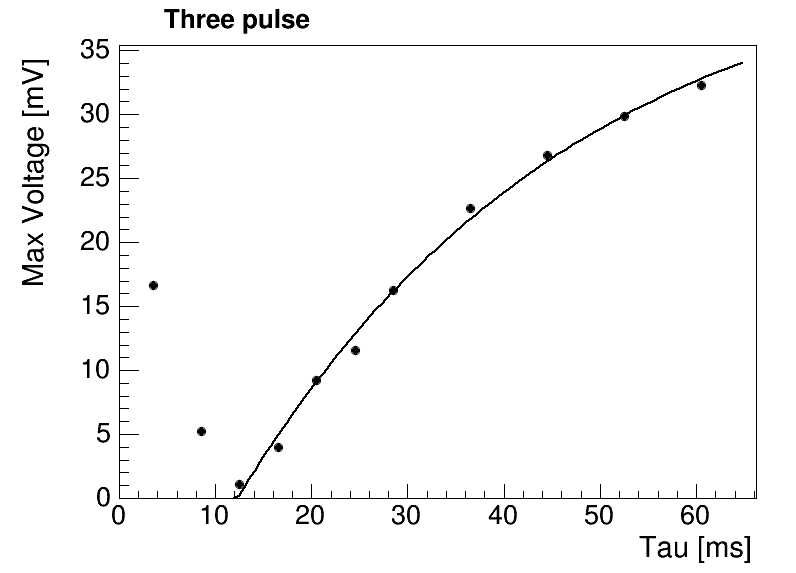
\includegraphics[width=6cm]{threePulse.png}
\caption{Spin echo amplitude as a function of delay time $\tau$ between first two pulses in the $\pi$-$\tau$-$\pi/2$-$\pi$ sequence. The uncertainties on each point are much larger than either FID-based method due to the uncertainty in measured spin echo height because of the relatively infrequent beat patterns. The nominal fit excluding the first three data points is shown.}
\label{fig:three}
\end{figure}

The measured $T_1$ for glycerine using the $\pi$-$\tau$-$\pi/2$-$\pi$ sequence was $25 \pm 23\mathrm{(fit}) \pm 86 \mathrm{(exc)}$.

\begin{table}[h]
\caption{\label{t:glyc} Summary of results from three methods of determining $T_1$ in glycerine. Note that all measurements are consistent, and that the first two FID-based methods have comparable uncertainties. }
\begin{tabular}{|c|c|}
\hline
Method & $T_{1} (ms)$ \\
\hline
$\pi/2$-$\tau$-$\pi/2$ & $30.9\pm4.5$ \\
\hline
$\pi$-$\tau$-$\pi/2$ & $27.1 \pm 6.2\mathrm{(fit}) \pm 0.92 \mathrm{(exc)}$ \\
\hline
$\pi$-$\tau$-$\pi/2$-$\pi$ & $25 \pm 23\mathrm{(fit}) \pm 86 \mathrm{(exc)}$ \\
\hline
\end{tabular}
\end{table}

A summary of the results from the above three measurements is given in Table \label{t:glyc}. All three measurements are consistent with each other. Averaging the results weighted by their uncertainties yields $T_1=29.6\pm3.7$ms, approximately 2$\sigma$ higher than the literature value of 20ms\cite{blo}. 

The $\pi$-$\tau$-$\pi/2$-$\pi$ measurement could be much improved by repetition with a more appropriate RF frequency, allowing for more frequent beat patterns and a more accurate determination of the spin echo amplitude. This would improve both the fit uncertainty and uncertainty based on how many points at low $\tau$ values are excluded.

Both the $\pi$-$\tau$-$\pi/2$-$\pi$ and $\pi$-$\tau$-$\pi/2$ could be vastly improved by either more data at longer $\tau$ to better establish the steady state measurement or implementation of a fit that takes into account the expected sharp turn over, which would require more data points to accurately fit an increased number of parameters. 

All three measurements could be improved by more data points both at different $\tau$ values and at each $\tau$ value. However, the third measurement is most likely to see marked improvement with a relatively small amount of further data.

The $\pi$-$\tau$-$\pi/2$ measurement sequence was repeated on three glycerine-water solutions of 30, 50, and 70 percent glycerine by weight. For each $\tau$, three measurements were taken with 32$\mu$s $\pi/2$ pulses and a repeat time of 500ms. Measurements were made for $\tau$s between 5ms and 100ms. The oscilloscope output was saved as a text file and processed. The measurement uncertainty was calculated and propagated as described for the $\pi/2$-$\tau$-$\pi/2$-$\pi$ pulse sequence. Each measurement uncertainty was on the order of 0.2-0.4mV. However, the scatter between measurements at the same $\tau$ was extremely large, resulting in much larger uncertainties on each combined measurement and a much messier signal curve.

\begin{table}[h]
\caption{\label{t:vis} Measured $T_{1}$ values for various concentrations of glycerine excluding either no, one, or two points. Note that all uncertainties are on the order of the $T_{1}$ value itself. Asterisks indicate that the fit had a MIGRAD status indicating a failure to converge. }
\begin{tabular}{|c|c|c|c|}
\hline
\% Glycerine & 30 & 50 & 70 \\
\hline
$T_{1,\mathrm{all}} (s)$ & $60 \pm 120$ & $140 \pm 370$ & $590 \pm 140$* \\
\hline
$T_{1,-1} (s)$                & $110 \pm 500$ & $35 \pm 34$ & $120 \pm 490$ \\
\hline
$T_{1,-2} (s)$                & $30 \pm 70$ & $26 \pm 43$ & $ 1500 \pm 770$* \\
\hline
\end{tabular}
\end{table}

For each viscosity, three fits were made to the recorded data: one to all points, one excluding the first point, and one excluding the first two points. The measured $T_{1}$ in each scenario with linearly propagated fit uncertainties for each viscosity are shown in Table \ref{t:vis}. The fit uncertainties are large enough that all other sources of uncertainty are neglected.

As indicated by the fit uncertainties, all measurements are consistent with zero. More data and data at longer delay times will improve the measurements to a certain extent. However, a measurement strategy such as the one described below for water is far more likely to produce significant results because these time constants are expected to be significantly longer than in pure glycerine.

For all methods described above, relaxation in the transverse plane will dominate all other effects at very long $\tau$ values. Measurements of the spin-lattice relaxation time in water, which has a much lower viscosity than glycerine and thus longer $T_1$, will necessitate measurements at very long $\tau$, making an accurate measurement of $T_{1}$ impossible. 

Instead, a modified version of a $\pi/2$-$\tau$-$\pi$ sequence is employed. The delay $\tau$ is held constant across all trials and the repeat time between sets of pulses is varied. For samples at thermal equilibrium before this pulse sequence, the first pulse produces a large FID as spins are rotated in to the plane. The second pulse then inverts all spins, creating a spin echo exactly $\tau$ after the second pulse. 

If the sample is not at thermal equilibrium before the pulse sequence is applied, both the FID and spin echo will be smaller than at thermal equilibrium. The expected spin height amplitude will go as $A(1-\mathrm{exp}(-t/T_{1}))$.

Two samples of water were analyzed, one with dissolved oxygen and one with dissolved nitrogen. For each repeat time and sample, three measurements were taken with 21$\mu$s $\pi/2$ pulses for dissolved nitrogen and 20$\mu$s for dissolved oxygen and a fixed $\tau = 2.0$ms. Repeat times up to 8 seconds were used for the dissolved nitrogen sample, but only up to 4.5 seconds for the dissolved oxygen sample. The oscilloscope output was saved as a text file and processed. 

The measurement uncertainty was calculated and propagated as described for the $\pi/2$-$\tau$-$\pi/2$-$\pi$ pulse sequence. For the three recorded waveforms in water with dissolved nitrogen with an 8s repeat time, there was another pulse sequence at the beginning of each waveform. For these three waveforms, the measurement uncertainty was taken to be the average measurement uncertainty for all other waveforms recorded with that sample. The measurement uncertainties ranged from 0.4-0.8mV. 

The spin echo amplitudes and uncertainties were calculated as described for the $\pi/2$-$\tau$-$\pi/2$-$\pi$ pulse sequence as the difference between the maximum and minimum point on the waveform after the RF pulses. The associated uncertainties were 0.8mV or less for each spin echo. 

The three measurements were averaged, and the overall uncertainty for each repeat time was taken as the standard deviation of the measurements added in quadrature with the calculated uncertainties based on waveform noise and spin echo amplitude extraction divided by the square root of the number of measurements.

The data was fit to a curve of the form $a-\mathrm{exp}(b\tau-c)$. The measured $T_{1}$ for water with dissolved nitrogen was $2.13\pm0.29$s. The measured $T_{1}$ for water with dissolved oxygen was $2.05\pm0.78$s. The two measurements are consistent with each other. Averaging the results weighted by their uncertainties yields $T_1=2.12\pm0.27$ms, consistent with the literature value of 2.3ms\cite{blo}. 

Note that the uncertainties in the spin echo amplitudes are much smaller in Fig \ref{fig:water} than in the $\pi$-$\tau$-$\pi/2$ sequence in glycerine (Fig \ref{fig:three}). The larger difference between the Larmor frequency for the water measurements compared to the glycerine measurements and more frequent beat patterns seem to have significantly improved the uncertainties related to the spin echo amplitude extraction.

As discussed above, the time constant in water with dissolved nitrogen is expected to be longer than the time constant with dissolved oxygen. This effect is not observed in this case. It is possible that the fit for the oxygenated water would change if longer repeat times were included, so the first-order improvement would be to make those measurements. However, the nitrogen sample was de-oxygenated an unknown amount of time ago, it is possible that the sample has since re-oxygenated and the measurements will be consistent regardless.

\begin{figure}[htb]
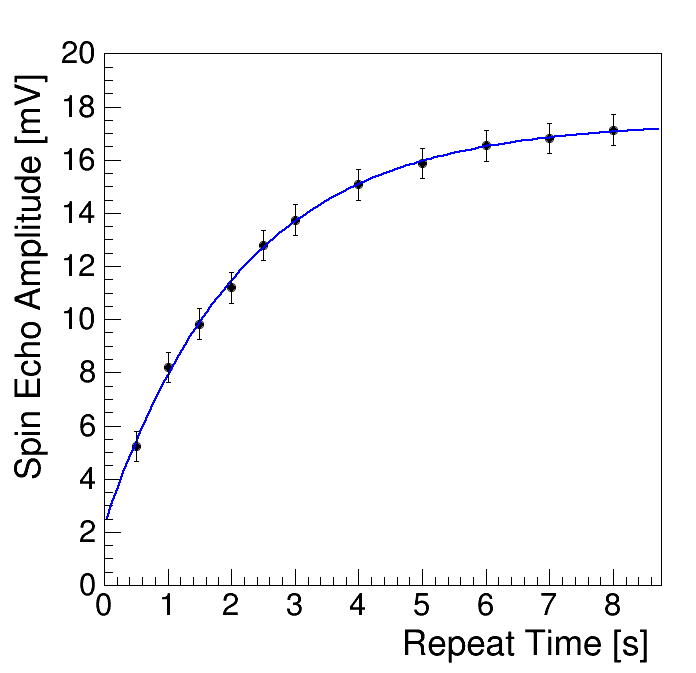
\includegraphics[width=6cm]{water_n2.png}
\caption{Spin echo amplitude as a function of repeat time for distilled water bubbled with diamagnetic N$_2$. }
\label{fig:water}
\end{figure}

To first order, the spin-lattice relaxation times are observed to increase with decreasing viscosity, from glycerine at $T_1=29.6\pm3.7$ms and water at $T_1=2.12\pm0.27$ms. No significant measurements were made at intermediate values of viscosity, so a more specific study of the viscosity-relaxation time cannot be made. 

We have additionally observed that an appropriate choice RF frequency is crucial to precision measurements of spin-lattice relaxation times and more generally all pulsed NMR measurements. In this case, our precision was vastly improved by moving from 2 kHz above the Larmor frequency of hydrogen to 10 kHz above. A more detailed study would likely find that there is some optimal distance that balances beat frequency with the overall response amplitude, which would improve future measurements of the spin-lattice relaxation times.

\begin{thebibliography}{3}

\bibitem{crc}
	"Nuclear Spins, Moments, and Other Data related to NMR Spectroscopy" from \emph{Handbook of Chemistry and Physics},
	94th ed.,
	2013.

\bibitem{ray}
	R. Freeman,
	"Spin-Lattice Relaxation" from \emph{A Handbook of Nuclear Magnetic Resonance},
	Longman,
	1988.

\bibitem{blo}
	N. Bloembergen,
	"Nuclear Magnetic Relaxation" reprinted in \emph{Nuclear Magnetic Relaxation},
	W.A. Benjamin,
	1961.

\end{thebibliography}

\end{document}
